\documentclass[9pt, aspectratio=169]{beamer}
\usepackage{FiraSans}
\usetheme{metropolis}
\usepackage[utf8]{inputenc}
\usepackage{amsmath}
\usepackage{amsfonts}
\usepackage{amssymb}
\usepackage{multicol}
\usepackage{tikz}
\usetikzlibrary{matrix}
\usepackage{xcolor}
\usepackage[T1]{fontenc} 
\usepackage[skins]{tcolorbox}
\author{Nicola Roman\`o - nicola.romano@ed.ac.uk}
\title{Image histogram}
\setlength{\fboxsep}{0pt}
\setbeamertemplate{caption}{\raggedright\insertcaption\par}
\setbeamertemplate {footline}{\begin{scriptsize}\hfill\insertframenumber ~of \inserttotalframenumber\kern1em\vskip5pt\end{scriptsize}}

%\setbeamercovered{transparent} 
%\setbeamertemplate{navigation symbols}{} 

\titlegraphic{\centering 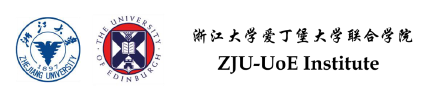
\includegraphics[scale=.5]{instituteLogo.png}}
\date{}

\AtBeginSection[]
{
  \begin{frame}<beamer>
    {Outline}
    \huge{\tableofcontents[currentsection]}
  \end{frame}
}

\begin{document}

\newtcolorbox{codebox}{enhanced,
    top=2pt,
    left=2pt,
    right=2pt,
    bottom=2pt,
    boxrule=0pt,
    leftrule=5pt,
    sharp corners,
    colback=gray!20,
    colframe=blue!60!black}

\begin{frame}
    \titlepage
\end{frame}

\begin{frame}
    {Learning objectives}
    \begin{columns}
        \begin{column}{0.8\textwidth}
            \begin{itemize}
                \item Define and produce an image histogram
                \item Use histograms to interpret image quality
                \item Apply point operations to manipulate image histograms
            \end{itemize}
        \end{column}
        \begin{column}{0.2\textwidth}
            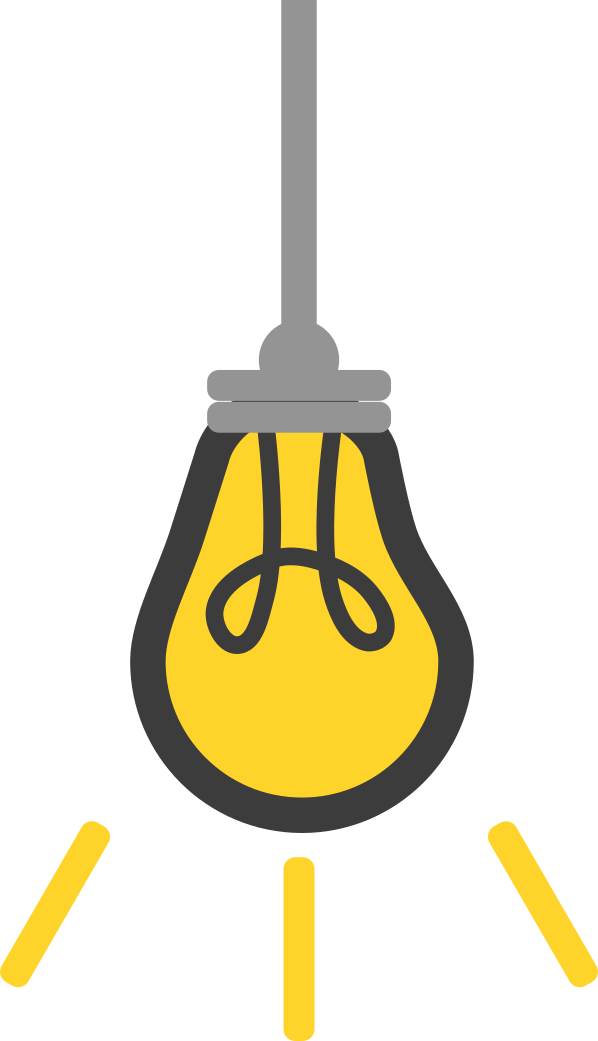
\includegraphics[angle=-30, origin=tr, width=1.5\textwidth]{lightbulb.png}
        \end{column}
    \end{columns}
\end{frame}

\section{Histograms}

\begin{frame}
    {What is a histogram?}
    "A histogram is an approximate representation of the distribution of numerical data." (\href{https://en.wikipedia.org/wiki/Histogram}{\small{\underline{Wikipedia}}})

    Given a variable $x$, in the interval $[x_{min}; x_{max}]$, we divide this interval (or a suitably larger one) into non-overlapping \textbf{bins} and count the number of values of x falling into each bin.\\
    Generally, we choose bins to be of equal size.
\end{frame}

\begin{frame}
    {Histogram example}
    Given $x = {5, 7, 10, 22, 35, 88, 26, 74, 22, 95}$

    We can choose the interval $[0; 99]$, and divide it into bins of size 10 $[0:9] [10; 19] \dots [90:99]$
    \pause
    \begin{columns}
        \begin{column}{0.5\textwidth}
            We now count the occurrences of $x$ in each bin.

            $$[0:9] \rightarrow 2$$
            $$[1:10] \rightarrow 1$$
            \dots
            and so on
        \end{column}
        \pause
        \begin{column}{0.5\textwidth}
            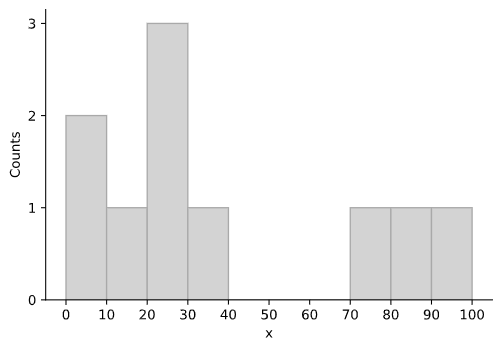
\includegraphics[width=\textwidth]{example_histogram.png}

            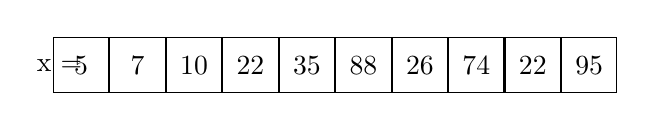
\begin{tikzpicture}[ampersand replacement=\&]
                \draw (0, 0) node {x =};
                \matrix [matrix of nodes, nodes={draw, minimum height=2em, minimum width=2em, anchor=center}, column sep=0] at (3.5, 0) {5 \& 7 \& 10 \& 22 \& 35 \& 88 \& 26 \& 74 \& 22 \& 95\\};
            \end{tikzpicture}

        \end{column}
    \end{columns}
\end{frame}

\begin{frame}
    {Histogram of an image}
    Images are just matrices, so we can count the occurrences of each pixel value in the image.

    \textbf{Example}

    An 8-bit image, 20 x 20

    \begin{columns}
        \begin{column}{0.5\textwidth}
            \begin{codebox}
                \texttt{> print(img.shape)\\
                    (20, 20)\\
                    >print(np.min(img))\\
                    0\\
                    >print(np.max(img))\\
                    100
                }
            \end{codebox}
            \only<2>
            {
                Maximum dynamic range [0, 255]

                We count the occurrences of each pixel with intensity between 0 and 255.
            }
        \end{column}
        \begin{column}{0.5\textwidth}
            \only<1>
            {
                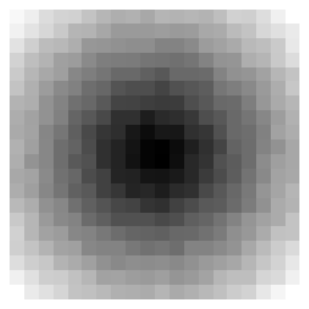
\includegraphics[width=.7\textwidth]{image_for_histo.png}
            }
            \only<2>
            {
                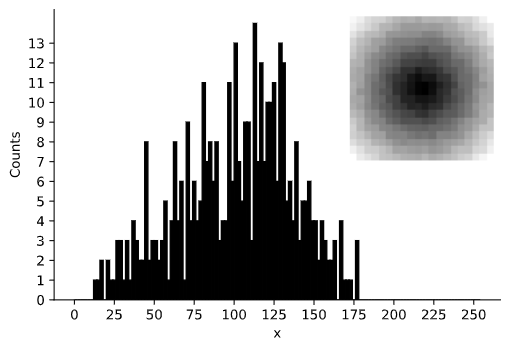
\includegraphics[width=\textwidth]{imagehist.png}

                \textbf{What can you tell about the image from looking at the histogram?}
            }
        \end{column}
    \end{columns}
\end{frame}

\begin{frame}
    {Logarithmic scale}
    Often it is useful to look at the histogram in logarithmic scale. This is particularly useful when images contain a lot of pixels of a specific intensity (e.g. cells on a black background).

    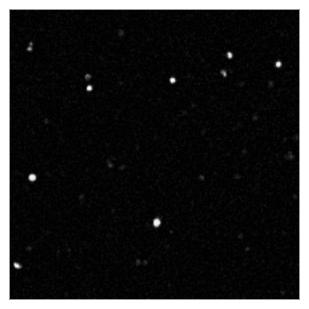
\includegraphics[height=.5\textheight]{pit_cells.png}
    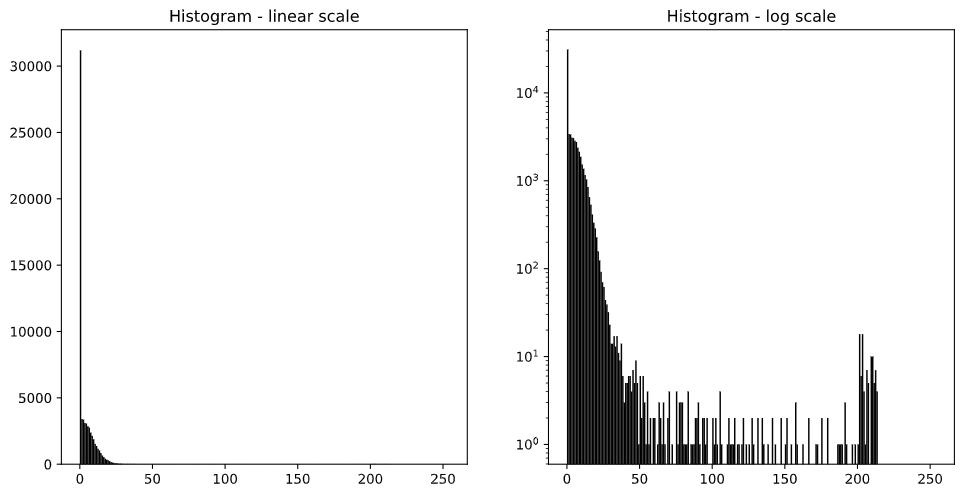
\includegraphics[height=.5\textheight]{pit_cells_histo_linear_vs_log.png}
\end{frame}

\begin{frame}
    {Histograms of RGB images}
    For RGB (or multi-channel) images, it makes sense to have a single histogram per channel

    \begin{columns}
        \begin{column}{0.5\textwidth}
            \begin{figure}
                \includegraphics[height=.5\textheight]{RetinaHnE.jpg}
                \caption{\small{\color{gray}{H\&E staining of retina (cell nuclei stained blue-purple and extracellular material stained pink)\newline Librepath - CC BY-SA 3.0}}}
            \end{figure}
        \end{column}
        \begin{column}{0.5\textwidth}
            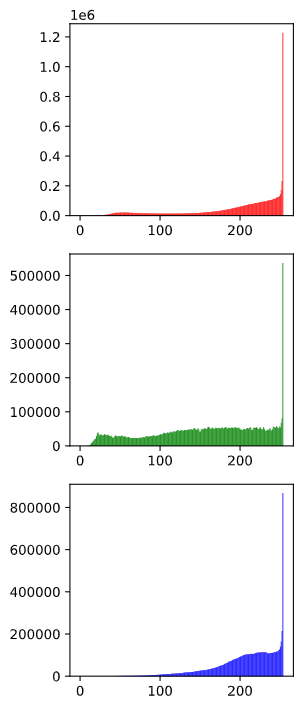
\includegraphics[height=.8\textheight]{RGBhisto.png}
            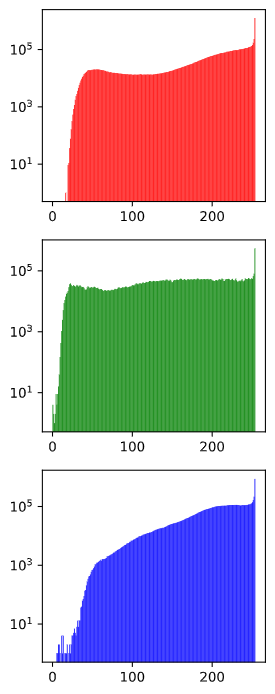
\includegraphics[height=.785\textheight]{RGBhistolog.png}

            \small{\color{gray}RGB histogram - left linear, right logarithmic.}
        \end{column}
    \end{columns}
\end{frame}

\begin{frame}
    {Histograms are destructive}
    It is important to remember that producing a histogram is a destructive operation. We can generate a histogram from an image, but cannot recreate the image from the histogram.

    \begin{figure}
        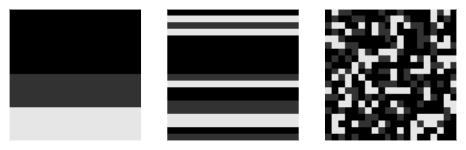
\includegraphics[width=.5\textwidth]{samehisto.png}
        \caption{These three images have the same histogram!}
    \end{figure}
\end{frame}

\begin{frame}
    {Drawing a histogram using Matplotlib}
    The Matplotlib \href{https://matplotlib.org/stable/api/_as_gen/matplotlib.pyplot.hist.html}{\underline{\texttt{hist}}} function makes it very easy to plot a histogram

    \begin{codebox}
        \texttt{import matplotlib.pyplot as plt\\
            img = io.imread("cells.tif")\\
            \\
            fig, ax = plt.subplots(1, 2, figsize=(12, 6))\\
            \# Linear\\
            ax[0].hist(img.ravel(), bins=range(255), color="black")\\
            ax[0].set\_title("Histogram - linear scale")\\
            \pause
            \# Log\\
            ax[1].hist(img.ravel(), bins=range(255), color="black", log=True)\\
            ax[1].set\_title("Histogram - log scale")\\
            plt.show()}
    \end{codebox}

    The \texttt{bins} parameter accepts either a sequence defining the bins edges, or a single value with the number of desired bins.
\end{frame}

\section {Brightness and contrast}

\begin{frame}
    {Brightness}
    The \textbf{brightness} of an image is the average intensity of all its pixels

    $$B(I) = \frac{1}{w*h}\sum_{r=1}^{h}\sum_{c=1}^{w}I(r,c)$$

    Where $w$ and $h$ are the width and height of the image, and $I(r,c)$ is the intensity of the pixel at row $r$ and column $c$.
    \pause
\end{frame}

\begin{frame}
{Brightness example}
\centering
\begin{figure}
    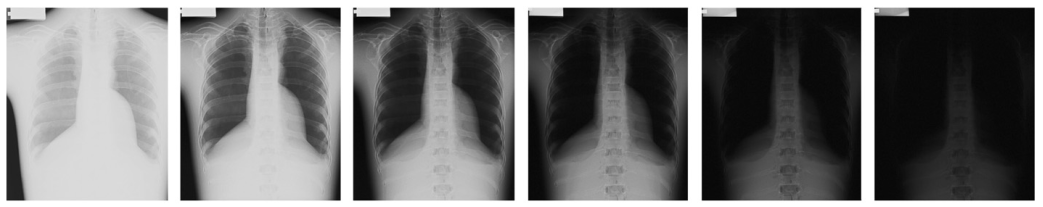
\includegraphics[width=\textwidth]{xray_brightness_Veldkamp_2009.png}
    \caption{\small{\color{gray}{Same X-ray, decreasing brightness - Image from Veldkamp et al., 2009}}}
\end{figure}
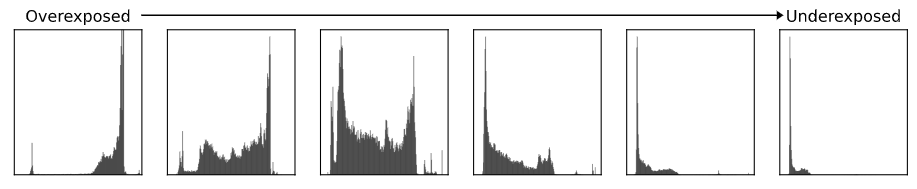
\includegraphics[width=\textwidth]{xray_brightness_Veldkamp_2009_histos.png}
Overexposed
\end{frame}
\begin{frame}
    {Contrast}
    \begin{columns}
        \begin{column}{.4\textwidth}
            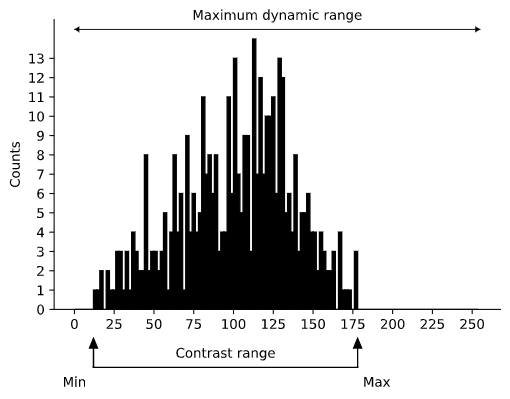
\includegraphics[width=\textwidth]{contrast range.png}
        \end{column}
        \begin{column}{.6\textwidth}
            \textbf{Contrast} is \textit{the difference in luminance or colour that makes an object distinguishable} (Wikipedia). It is a measure of the relationship between light and dark pixels in an image. 
            \pause
            Many different definitions in the literature (see Peli, \textit{J. Opt. Soc. Am. A}, 1990)
            
            \textbf{Weber contrast} (range $0 \rightarrow \infty$)

            $$\frac{I_{obj}-I_{bg}}{I_{bg}}$$

            \textbf{Michelson contrast} (range $0 \rightarrow 1$)
            $$\frac{I_{max}-I_{min}}{I_{max}+I_{min}}$$

            \textbf{RMS contrast}
            $$\sqrt{\frac{1}{n-1}\sum_{i=1}^{n}(x_i-\bar{x})^2}$$ where $x$ is the normalised intensity $0 \leq x \leq 1$

        \end{column}
    \end{columns}
\end{frame}

\section {Point operations}

\begin{frame}
{Histogram equalization}
\end{frame}

\begin{frame}
{Histogram matching}
\end{frame}
\end{document}

